\providecommand{\main}{../../../..}
\documentclass[\main/dresen_thesis.tex]{subfiles}

\begin{document}
  \label{sec:colloidalCrystals:nanoparticle:tem}
  \begin{figure}[!htbp]
    \centering
    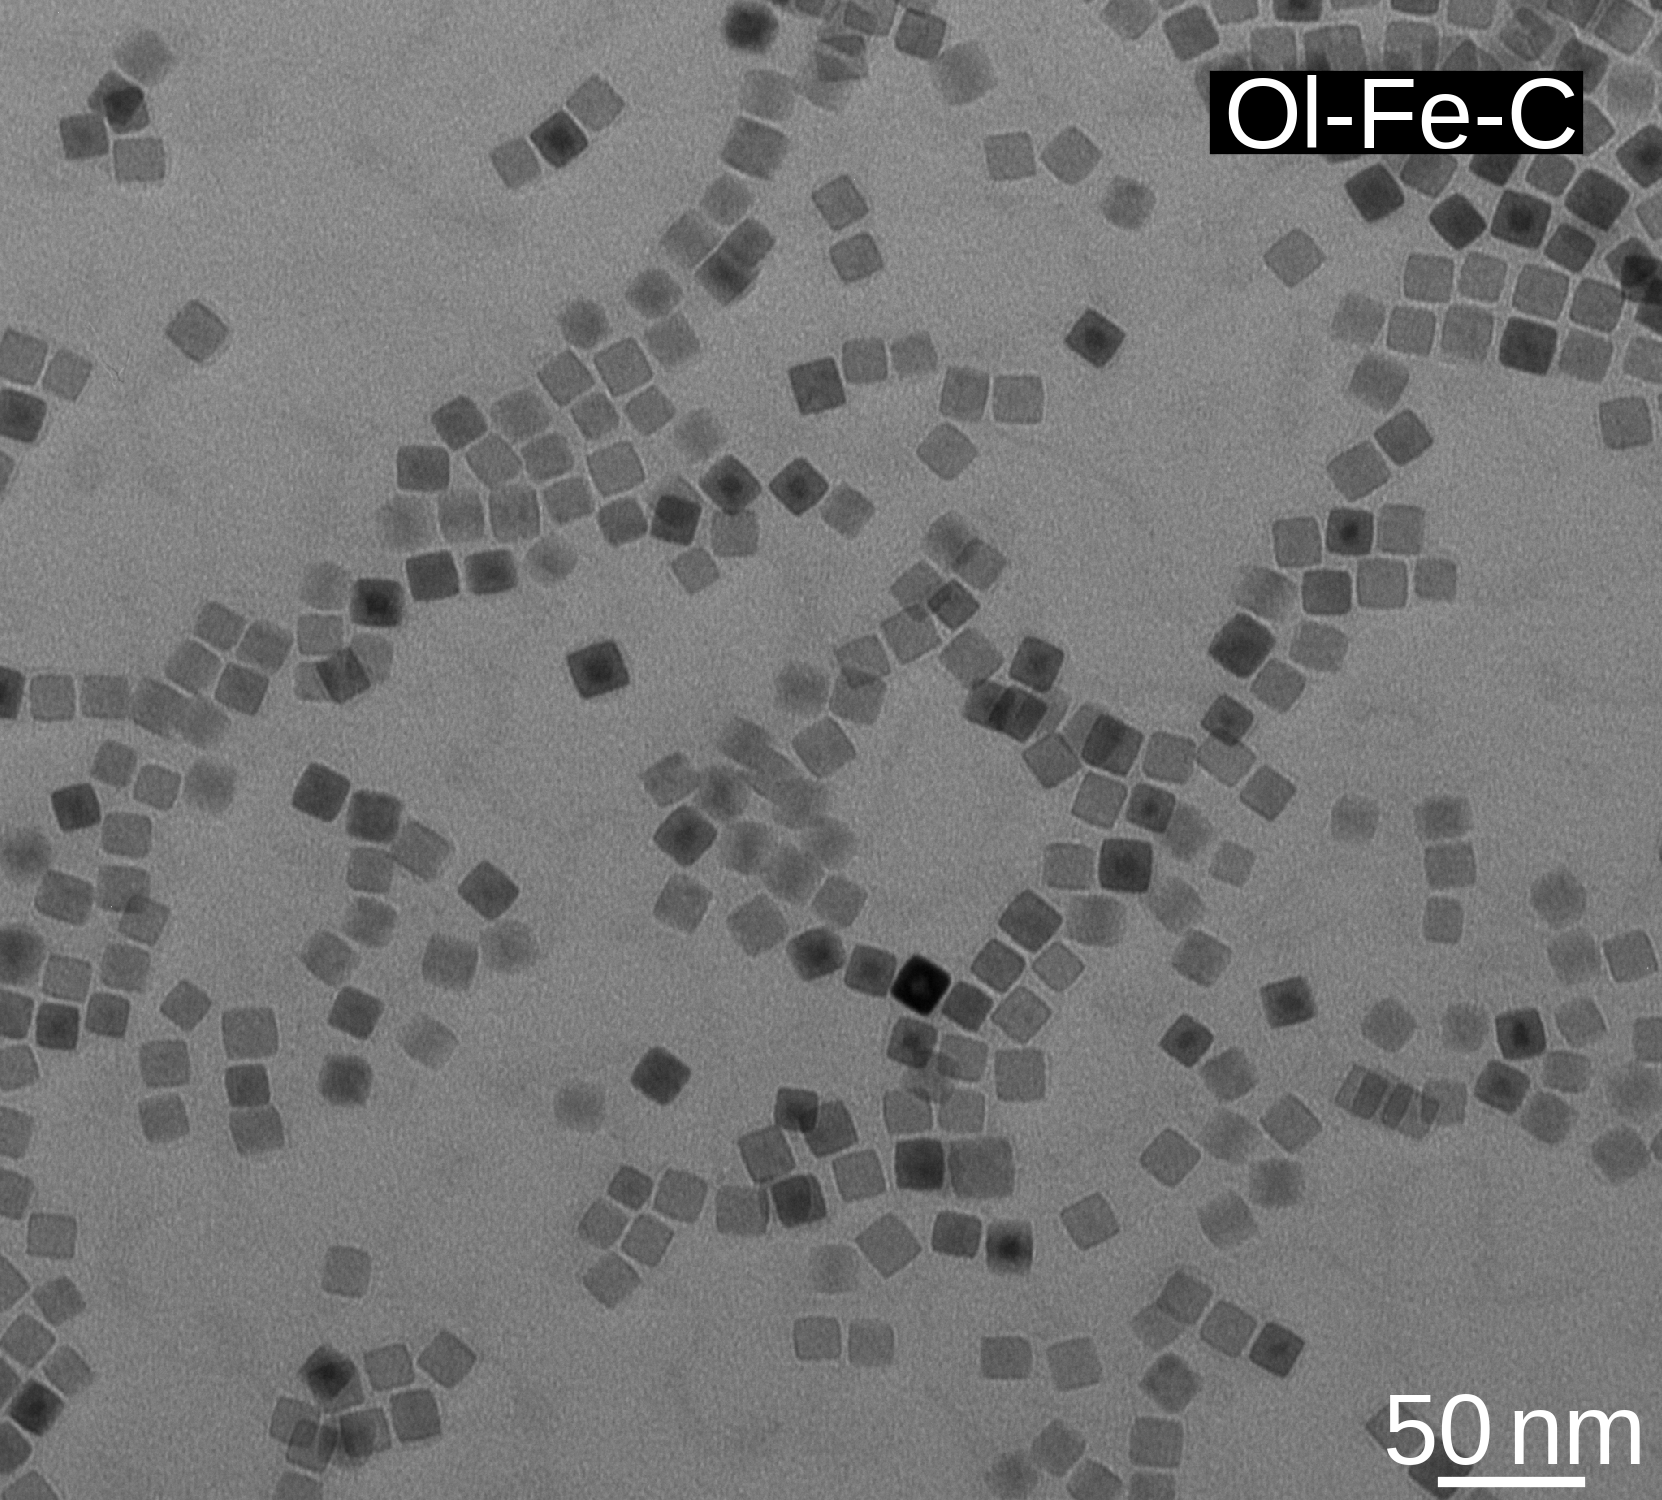
\includegraphics{colloidalCrystals_TEM_Ol_Fe_C}
    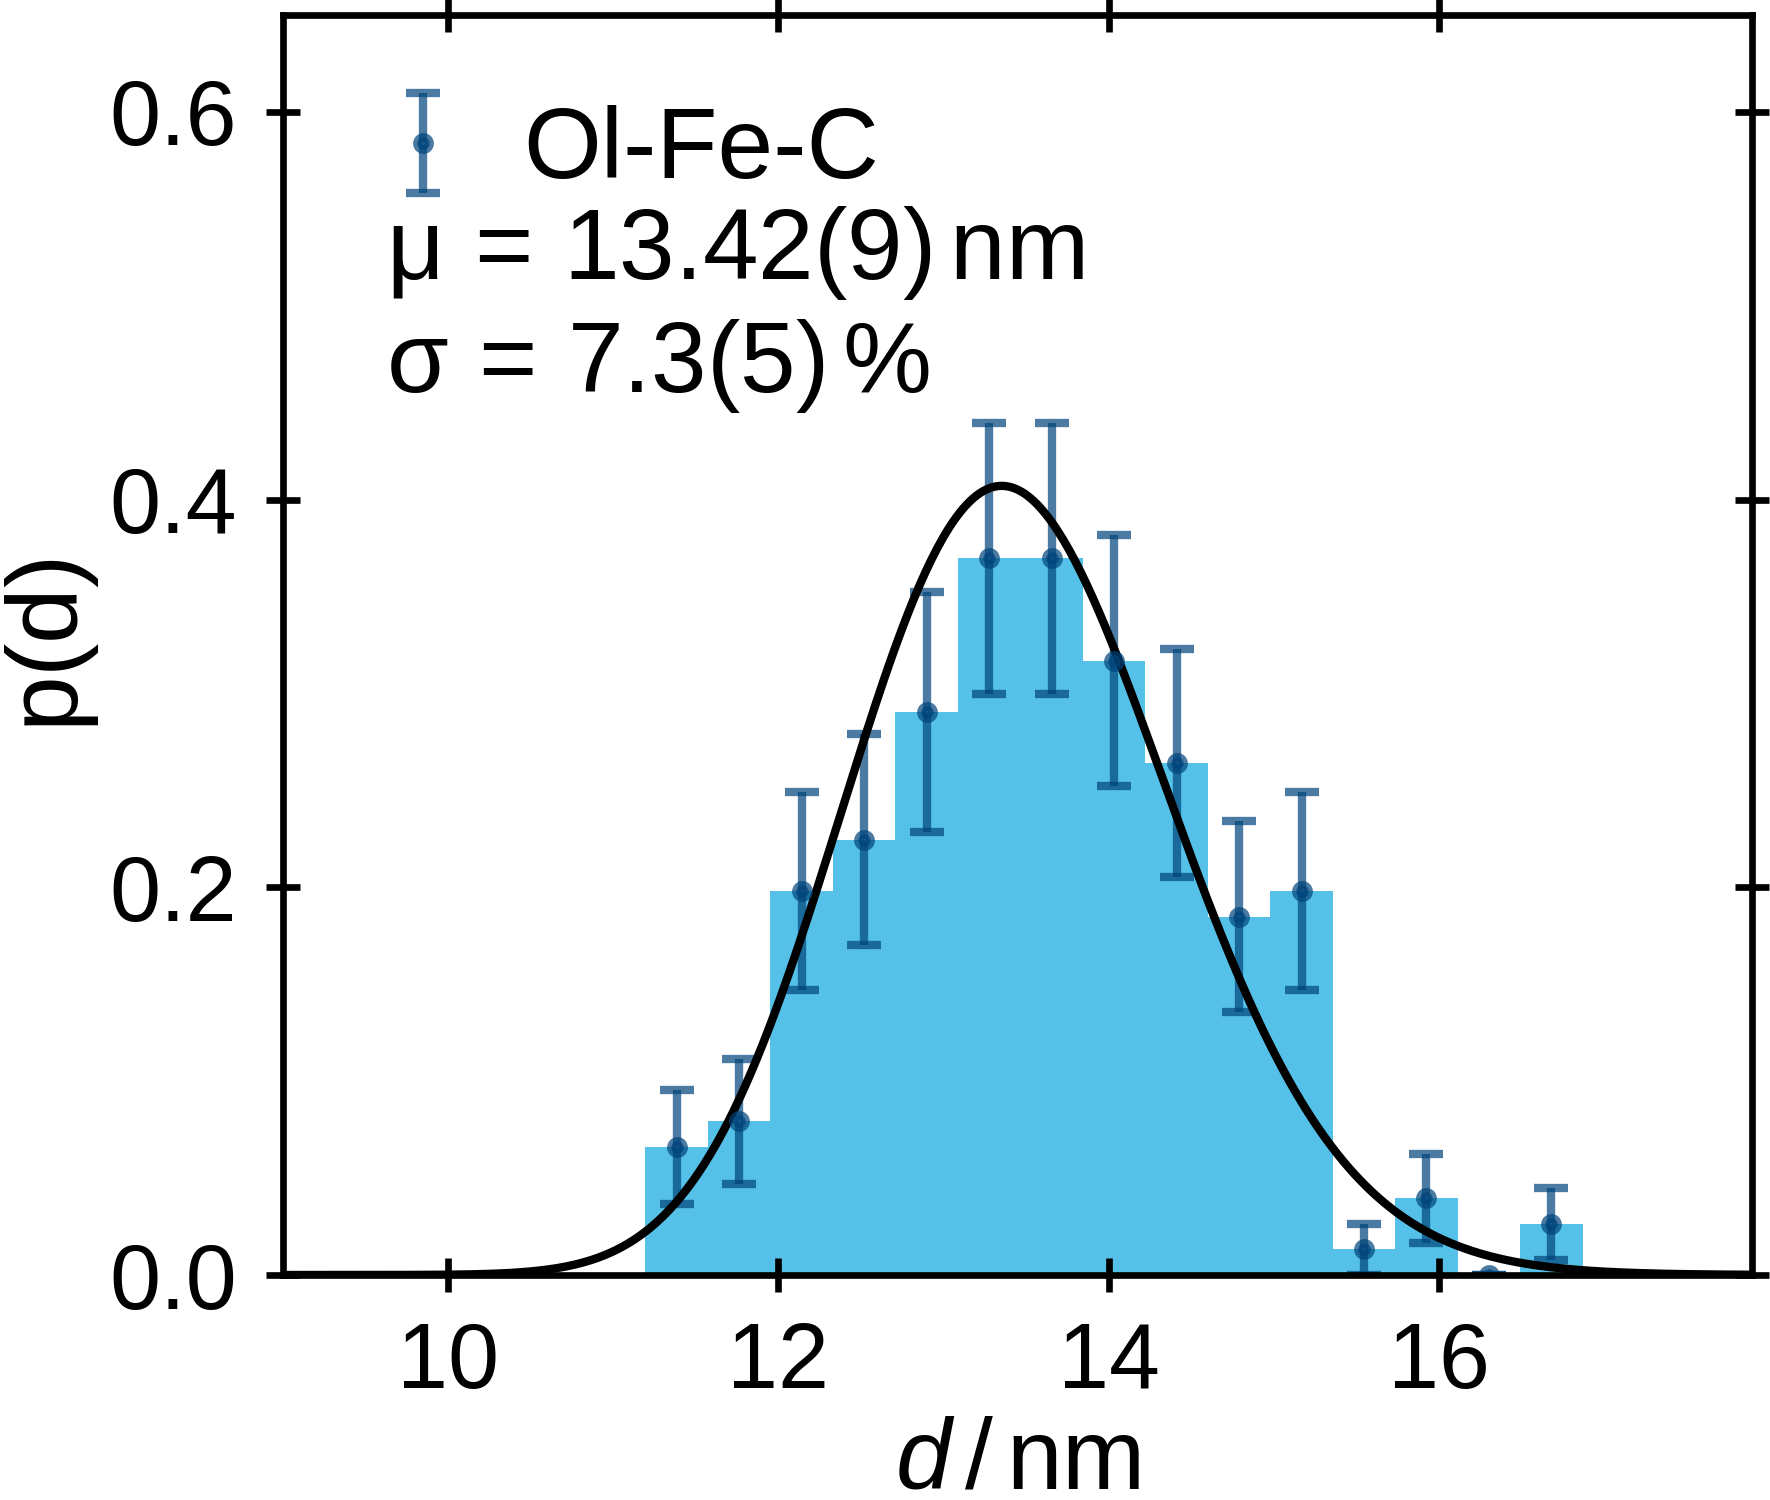
\includegraphics{colloidalCrystals_TEM_Ol_Fe_C_sizeDist}
    \caption{\label{fig:colloidalCrystals:nanoparticle:tem}TEM micrograph of Ol-Fe-C (left) and the particle size distribution of the nanocube's edge length (right).}
  \end{figure}

  In \reffig{fig:colloidalCrystals:nanoparticle:tem}, an exemplary micrograph of Ol-Fe-C is shown.
  The micrograph confirms the cubic shape of the nanoparticles and suggests a homogeneous size distribution and morphology.
  Furthermore, within multiple nanocubes darker core areas can be spotted across the micrograph.
  To estimate the average edge length of the nanocubes, a histogram of manually measured edge lengths is shown and fit with a log-normal distribution.

  The average edge length is determined to $13.42(9) \unit{nm}$, with a log-normal width of $7.3(5) \unit{\%}$.
  In comparison to the nanocubes discussed previously in \refch{ch:monolayers}, this size is slightly larger but in a similar order of magnitude.

  The darker areas observed in the micrograph can be alludes to the core-shell structure of the nanocubes.
  As the particles are synthesized from iron oleate in 1-octadecene, a w\"ustite core and magnetite/maghemite shell is expected for the nanoparticles as it is commonly observed in literature \cite{Wetterskog_2013_Anoma}.
\end{document}